
%%%%
% TODO macros
\newcommand{\MK}[1]{\todo[color=orange!30]{TODO: #1}}
\newcommand{\MP}[1]{\todo[color=blue!30]{TODO: #1}}
\newcommand{\hltt}[1]{\begin{center}\fbox{\color{green}\large{#1}}\end{center}}

%%%%
% Text Decorations
\newcommand\BrText[2]{%
  \par\smallskip
   \noindent\makebox[\textwidth][r]{$\text{\scriptsize #1}\left\{
    \begin{minipage}{\textwidth}
    #2
    \end{minipage}
  \right.\nulldelimiterspace=0pt$}\par\smallskip
}

%%%%
% List of contributions
\newcounter{contrib}
\newcommand{\contribnum}[0]{\stepcounter{contrib}{\arabic{contrib}}.~}
\newcommand{\contribution}[1]{\smallskip\noindent\textbf{{#1.}\xspace}}

%%%%
% A symbol for Coq-verified theorems.
\newcommand{\BareCoqSymbol}{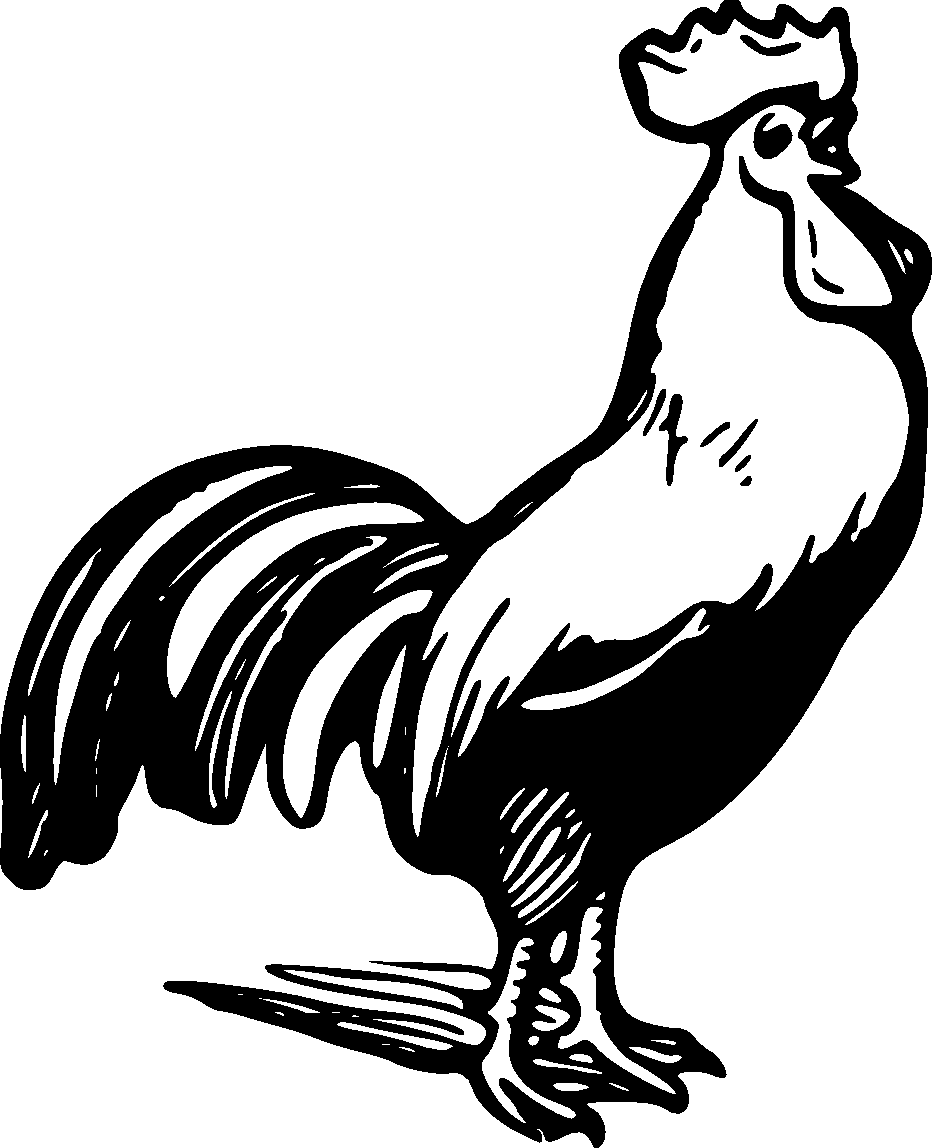
\includegraphics[height=0.9em]{coq.pdf}}
\newcommand{\CoqSymbol}{\raisebox{-.2ex}{\BareCoqSymbol\,}}
\newcommand{\Coqed}{\hfill\CoqSymbol}

\newcommand{\BareInvCoqSymbol}{
\includegraphics[height=0.9em]{inv_coq.png}}
\newcommand{\InvCoqSymbol}{\raisebox{-.2ex}{\BareInvCoqSymbol\,}}

%%%%
% Colors
\newcommand{\neutcol}[0]{black}
\newcommand{\stlccol}[0]{RoyalBlue}
\newcommand{\irccol}[0]{Apricot}
\newcommand{\ulccol}[0]{RedOrange}
\newcommand{\objcol}[0]{Emerald} %CarnationPink}
\newcommand{\commoncol}[0]{black}

\newcommand{\col}[2]{\ensuremath{{\color{#1}{#2}}}}

\newcommand{\com}[1]{\ensuremath\mathit{\col{\neutcol}{#1}}}
\newcommand{\src}[1]{\ensuremath\mathsf{\col{\stlccol}{#1}}}
\newcommand{\irl}[1]{\ensuremath\mathit{\col{\irccol}{#1}}}
\newcommand{\trg}[1]{\ensuremath\mathbf{\col{\ulccol}{#1}}}
\newcommand{\obj}[1]{\ensuremath\mathtt{\col{\objcol}{#1}}}
